\documentclass[a4paper,12pt,twocolumn]{article}
\usepackage{graphicx}
\usepackage[margin=0.5in]{geometry}
\usepackage[cmex10]{amsmath}
\usepackage{array}
\usepackage{gensymb}
\usepackage{booktabs}
\usepackage{tabularx}
\title{Conic Assignment}

\author{Ginna Shreyani- FWC22006}
\date{October 2022}
\providecommand{\norm}[1]{\left\lVert#1\right\rVert}
\providecommand{\abs}[1]{\left\vert#1\right\vert}
\let\vec\mathbf
\newcommand{\myvec}[1]{\ensuremath{\begin{pmatrix}#1\end{pmatrix}}}
\newcommand{\mydet}[1]{\ensuremath{\begin{vmatrix}#1\end{vmatrix}}}
\providecommand{\brak}[1]{\ensuremath{\left((#1\right)}}
\begin{document}
\maketitle											
\section{Problem:}
Minimize Z=x+2y subject to
\begin{align*}
&2x+3y\ge3,x+2y\ge6,x,y\ge0.
\end{align*}
\maketitle
\section{Solution:}
The given equations are
\begin{align*}
&2x+y\ge3\\
&x+2y\ge6\\
&x,y\ge0\\
\end{align*}
\begin{figure}[h]
     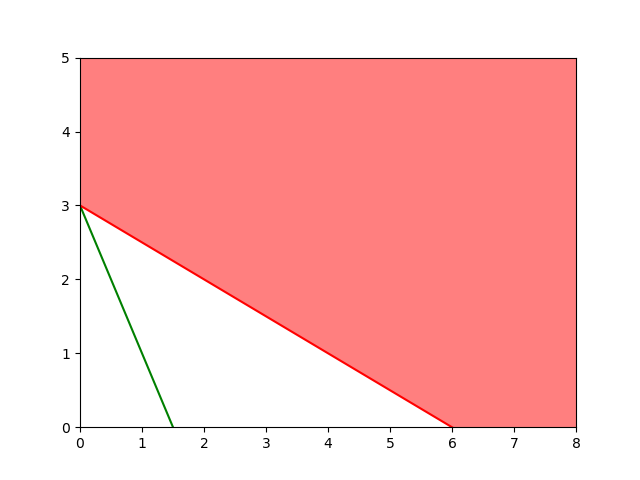
\includegraphics[width=\linewidth]{figures/optimize.png}
\end{figure}
By solving the above equations we get that feasible region of  these two equations is unbounded.Here, the red unbounded region is the feasible region of the above given equations. Here the feasible region is unbounded, so the minimum value of $\vec{Z}$ is found by finding the corner points.\\
\begin{align}
	P = \min_{\vec{x}}\myvec{1 &2}\vec{X}
	\\
	\myvec{2 &1 \\ 1 & 2} \vec{X}\succeq \myvec{3 \\ 6}
	\\
	\vec{x},\vec{y} \succeq \vec{0}
\end{align}
 %Graphical solution:} 
				the feasible region vertices are
\begin{align}
\myvec{0 \\ 3 },
\myvec{6 \\ 0}
\end{align}
with respective minium value
\begin{align}
	\myvec{1 &2}\myvec{0 \\ 3} &= 6 \\
	\myvec{1 &2}\myvec{6 \\ 0} &= 6 \\
	%\myvec{30 &20}\myvec{4 \\ 12} &= 360
\end{align}
Thus, the minimum value of Z is 6 along the line $\myvec{1 & 2}\vec{X}=\myvec{6 \\ 0}$.
\end{document}

